\documentclass{article} % For LaTeX2e
% We will use NIPS submission format
\usepackage{nips13submit_e,times}
% for hyperlinks
\usepackage{hyperref}
\usepackage{url}
% For figures
\usepackage{graphicx} 
\usepackage{subfigure} 
% math packages
\usepackage{amsmath}
\usepackage{amsfonts}
\usepackage{amsopn}
\usepackage{ifthen}
\usepackage{natbib}

\title{Project-I by Group Sao Paulo}

\author{
Damien Engels\\
EPFL \\
\texttt{damien.engels@epfl.ch} \And No\'emie Jaquier\\
EPFL \\
\texttt{noemie.jaquier@epfl.ch} \\
}

% The \author macro works with any number of authors. There are two commands
% used to separate the names and addresses of multiple authors: \And and \AND.
%
% Using \And between authors leaves it to \LaTeX{} to determine where to break
% the lines. Using \AND forces a linebreak at that point. So, if \LaTeX{}
% puts 3 of 4 authors names on the first line, and the last on the second
% line, try using \AND instead of \And before the third author name.

\nipsfinalcopy 

\begin{document}

\maketitle

\begin{abstract}
In this report, ...
\end{abstract}

\section{Regression}
\subsection{Data Description}
Our regression-data contains $N=2800$ train-examples and $N=1200$ test-data. The train-data are composed of input and output variables $X$ and $y$. Each input $x_n$ has a dimensionality $D=70$ with 60 real-valued variables, 1 binary variable, 5 and 4 categorical variables with respectively 3 and 4 categories. The output of our test-data is not observed. Our goal is then to predict $y$ for all test-examples and to give an approximation of the test-error.

\subsection{Data Visualization and Cleaning}
To visualise our data, we plot histograms to see the distribution of $y$ and of each dimension of X. The input data is not centred, so that we need to normalise it. 

Figure \todo{ADD FIGURE} shows the histogram of the output variable. We see that the data are split in three bursts of different sizes : a large amount of the data have small output values and only a small part have the highest values. Figure \todo{ADD FIGURE} shows histograms of two interesting dimensions of $X$. As all others real-valued variables seem to have sort of Gaussian distributions, we can see that those are split in two bursts. By plotting $y$ in function of each of these variables, as shown in Figure \todo{ADD FIGURE}, we can see that $y$ is highly correlated with dimensions $6$ and $55$ of $X$. The output-data can thus be separated in three clusters by looking at $x_n(6)$ ans $x_n(55)$ for each data.

We also computed the eigenvalues of the matrix $X^T X$. As ten eigenvalues are smaller than $10^{-10}$, we will need to transform $X$ to remove those small eigenvalues or to use methods such as ridge regression to lift them. 

%\begin{figure}[!h] % !t
%\center
%\subfigure[Boxplot of real-valued $\mathbf{X}$. Data is not centered and therefore we normalize it.]{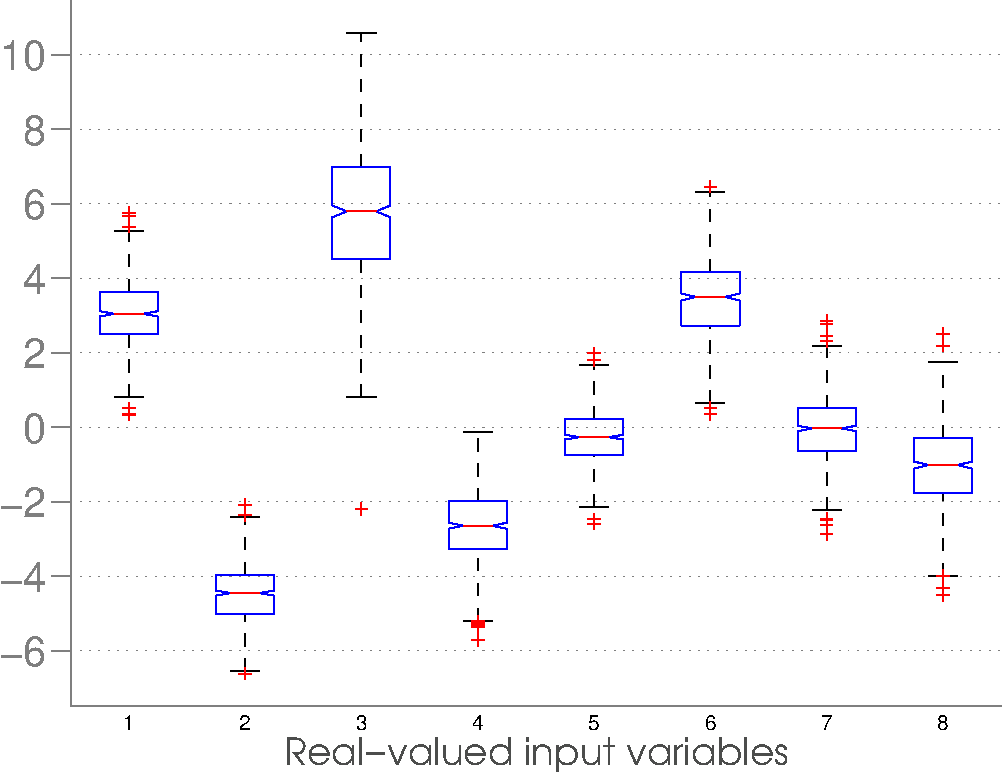
\includegraphics[width=2.5in]{figures/boxplotX.pdf} \label{fig:boxplotX}}
%\hfill
%\subfigure[Histogram of $\mathbf{y}$. We can clearly see two outliers.]{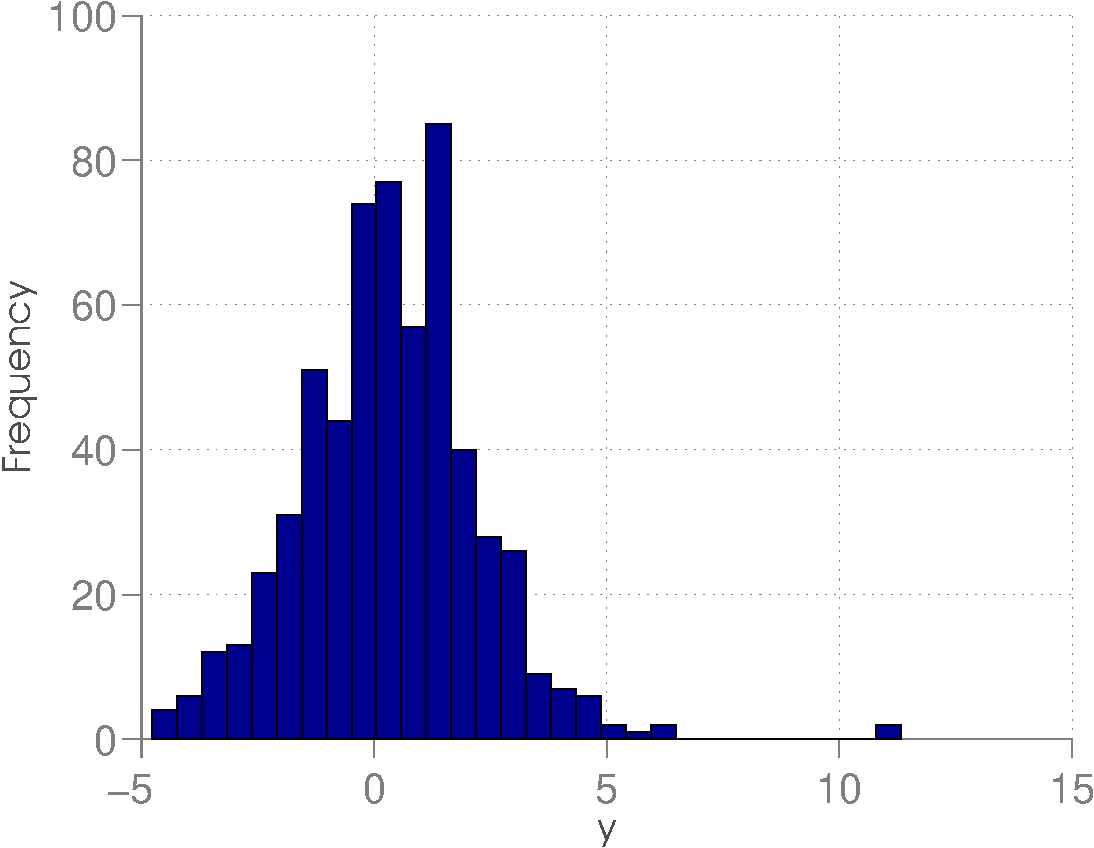
\includegraphics[width=2.5in]{figures/histY.pdf} \label{fig:histY}}
%\caption{}
%\end{figure}

\subsection{Clustering and Feature Transformations}

\subsection{Methods}
We applied least-squares and ridge regression to this dataset...

\subsection{Feature transformations}
We tried several feature transformations...

\section{Classification}
\subsection{Data Description}
\subsection{Data Visualization and Cleaning}
\subsection{Logistic Regression}


\section{Summary}
In this report, we ...


\subsubsection*{Acknowledgments}
...

\subsubsection*{References}

\end{document}
